\section{Introduction}

The structure of a physical database is organized as illustrated below:
\begin{figure}[H]
    \centering
    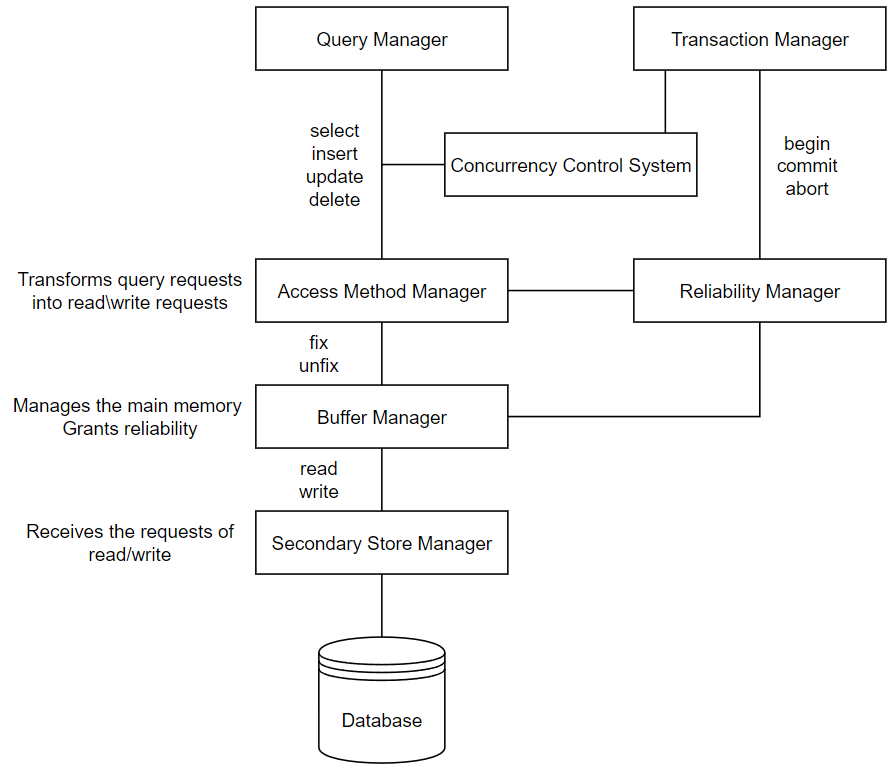
\includegraphics[width=0.5\linewidth]{images/structure.png}
    \caption{Architecture of a DBMS}
\end{figure} 

Data are primarily stored in files on secondary memory due to considerations of size and persistence.
Data in secondary memory becomes usable only when loaded into main memory through an I/O operation.
The storage units are referred to as:
\begin{itemize}
    \item \textit{Block}, when in secondary memory, with a fixed length of a few kilobytes.
    \item \textit{Page}, when in primary memory, assuming a size equivalent to that of blocks.
\end{itemize}
The time required for reading a block from a disk depends on the storage technology: Hard Disk Drive or Solid State Drive.

\paragraph*{Hard disk drive}
Hard Disk Drives involve multiple disks stacked and rotating at a constant angular speed.
A head stack, mounted on an arm, moves radially to reach tracks at various distances from the rotation axis, called spindle.
A specific sector is accessed by waiting for it to pass under one of the heads.
Multiple blocks can be accessed simultaneously (equal to the number of heads/disks).
\begin{figure}[H]
    \centering
    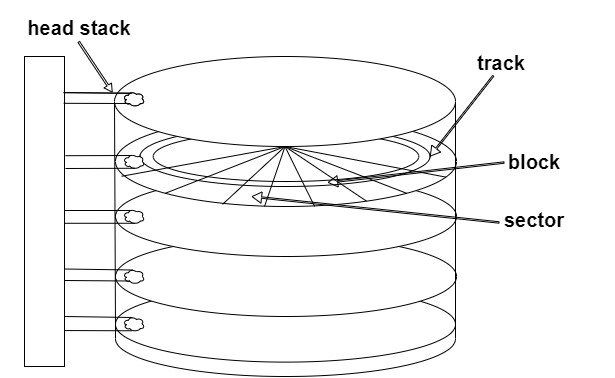
\includegraphics[width=0.35\linewidth]{images/hdd.png}
    \caption{Structure of a Hard Disk Drive}
\end{figure} 

\paragraph*{Access time} 
The secondary memory access time comprises:
\begin{itemize}
    \item \textit{Seek time} (8-12ms): head positioning on the correct track. 
    \item \textit{Latency time} (2-8ms): disc rotation on the correct sector. 
    \item \textit{Transfer time} ($\thicksim$ 1ms): data transfer.
\end{itemize}
The cost of accessing secondary memory is four orders of magnitude higher than that of main memory.
In many applications, the cost depends solely on the number of accesses to secondary memory.
The cost of a query is closely related to the amount of data read (moved) from secondary memory.

\paragraph*{File System} 
The File System, the operating system layer managing secondary memory, is utilized minimally by the DBMS.
DBMS directly manage file organization, both in data distribution within blocks and internal block structures. 
Additionally, a DBMS may control the physical allocation of blocks on the disk to optimize access time or enhance reliability.